\begin{spacing}{1}

    \chapter*{Abstract}

\end{spacing}

\begin{wrapfigure}{r}{0.3\textwidth}

    \begin{center}

        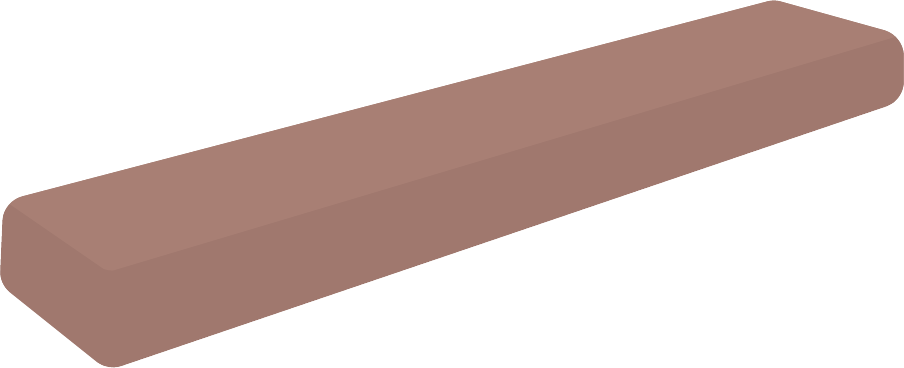
\includegraphics[width=0.2\textwidth]{pics/abstract_picture_1}

    \end{center}

\end{wrapfigure}

Beam VR is a project which aims to give an immersive experience of height.
It consists of a scene on top of a building with a plank, which protrudes from this building.
To increase the immersion we use virtual reality combined with the physical reality (Augmented Virtuality).
In particular the plank exists in the virtual as well as in the physical reality.

With a realistic environment including cars, high skyscrapers and classic new york city sounds we optimize the immersion of the reality.
The objective of the simulation is balancing on the beam without falling off.
Furthermore, the scene can be experienced in three different maps, namely Night, Day and Apocalypse.

\newpage

\begin{spacing}{1}

    \chapter*{Zusammenfassung}

\end{spacing}

\begin{wrapfigure}{r}{0.3\textwidth}

    \begin{center}

        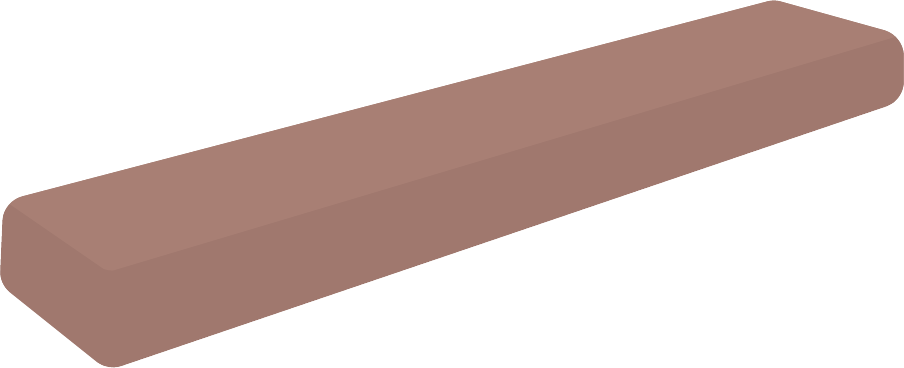
\includegraphics[width=0.2\textwidth]{pics/abstract_picture_1}

    \end{center}

\end{wrapfigure}

Beam VR ist ein Projekt, das darauf abzielt, ein immersives Höhenerlebnis zu vermitteln.
Es besteht aus einer Szene auf einem Gebäude mit einem Brett, das aus diesem Gebäude herausragt.
Um die Immersion zu steigern, verwenden wir Virtual Reality in Kombination mit der physischen Realität (Augmented Virtuality).
Insbesondere das Brett existiert sowohl in der virtuellen als auch in der physischen Realität.

Mit einer realistischen Umgebung aus Autos, hohen Wolkenkratzern und klassischen New-York-City-Sounds optimieren wir das Eintauchen in die Realität.
Ziel der Simulation ist es, auf dem Balken zu balancieren, ohne herunterzufallen.
Darüber hinaus kann die Szene in drei verschiedenen Karten erlebt werden, nämlich Night, Day und Apocalypse.
